\documentclass[letterpaper,12pt]{article}
\usepackage{array}
\usepackage{threeparttable}
\usepackage{geometry}
\geometry{letterpaper,tmargin=1in,bmargin=1in,lmargin=1.25in,rmargin=1.25in}
\usepackage{fancyhdr,lastpage}
\pagestyle{fancy}
\lhead{}
\chead{}
\rhead{}
\lfoot{}
\cfoot{}
\rfoot{\footnotesize\textsl{Page \thepage\ of \pageref{LastPage}}}
\renewcommand\headrulewidth{0pt}
\renewcommand\footrulewidth{0pt}
\usepackage[format=hang,font=normalsize,labelfont=bf]{caption}
\usepackage{listings}
\lstset{frame=single,
  language=Python,
  showstringspaces=false,
  columns=flexible,
  basicstyle={\small\ttfamily},
  numbers=none,
  breaklines=true,
  breakatwhitespace=true
  tabsize=3
}
\usepackage{amsmath}
\usepackage{amssymb}
\usepackage{amsthm}
\usepackage{harvard}
\usepackage{setspace}
\usepackage{float,color}
\usepackage[pdftex]{graphicx}
\usepackage{hyperref}
\hypersetup{colorlinks,linkcolor=red,urlcolor=blue}
\theoremstyle{definition}
\newtheorem{theorem}{Theorem}
\newtheorem{acknowledgement}[theorem]{Acknowledgement}
\newtheorem{algorithm}[theorem]{Algorithm}
\newtheorem{axiom}[theorem]{Axiom}
\newtheorem{case}[theorem]{Case}
\newtheorem{claim}[theorem]{Claim}
\newtheorem{conclusion}[theorem]{Conclusion}
\newtheorem{condition}[theorem]{Condition}
\newtheorem{conjecture}[theorem]{Conjecture}
\newtheorem{corollary}[theorem]{Corollary}
\newtheorem{criterion}[theorem]{Criterion}
\newtheorem{definition}[theorem]{Definition}
\newtheorem{derivation}{Derivation} % Number derivations on their own
\newtheorem{example}[theorem]{Example}
\newtheorem{exercise}[theorem]{Exercise}
\newtheorem{lemma}[theorem]{Lemma}
\newtheorem{notation}[theorem]{Notation}
\newtheorem{problem}[theorem]{Problem}
\newtheorem{proposition}{Proposition} % Number propositions on their own
\newtheorem{remark}[theorem]{Remark}
\newtheorem{solution}[theorem]{Solution}
\newtheorem{summary}[theorem]{Summary}
\newcommand{\R}{\mathbb{R}}
%\numberwithin{equation}{section}
\bibliographystyle{aer}
\newcommand\ve{\varepsilon}
\newcommand\boldline{\arrayrulewidth{1pt}\hline}


\begin{document}

\begin{flushleft}
  \textbf{\large{Problem Set \#2 Part 1}} \\
  OSM Lab, Professor Stachurski  \\
  Dan Ehrlich
\end{flushleft}

\vspace{3mm}

\noindent\textbf{Problem 1}
First checking for the spectral radius condition, the largest eigenvalue of matrix A has a value of $0.965538166352 < 1$ so the spectral radius condition holds and the equation $x = A x + b$ has a unique solution. Solving for $x$ using both matrix algebra and successive approximations we get that:
\[ x =
\begin{bmatrix}
 -0.89552239 \\
  13.34328358\\
  45.64179104
\end{bmatrix}
\]\\

\noindent\textbf{Problem 2}
In a standard job search model, we have that $\bar w$ should satisfy 
$$
    \bar w
    = c (1-\beta) + \beta
    \sum_{k=1}^K \max \left\{
        w_k ,\, \bar w
    \right\}
    \, p_k
$$
We need to show that $T(x): \R_+ \to \R_+$  is a contraction mapping where $T(x) =  c (1-\beta) + \beta \sum_{k=1}^K \max \left\{w_k ,\, x\right\} \, p_k$. Consider
\begin{equation*}
\begin{aligned}
 |T(x)- T(y)| & =  \big |c (1-\beta) + \beta \sum_{k=1}^K \max \left\{w_k ,\, x\right\} \, p_k - c (1-\beta) + \beta \sum_{k=1}^K \max \left\{w_k ,\, y\right\} \, p_k \big |=\\
& = \beta \big |\sum_{k=1}^K \max \left\{w_k ,\, x\right\}p_k - \sum_{k=1}^K \max \left\{w_k ,\, y\right\} \, p_k \big | = \\
& = \beta \big |\sum_{k=1}^K (\max \left\{w_k ,\, x\right\} -  \max \left\{w_k ,\, y\right\} \,) p_k \big |  \\
& \leq \beta \sum_{k=1}^K \big |(\max \left\{w_k ,\, x\right\} -  \max \left\{w_k ,\, y\right\} \,) \big |p_k   \\
& \leq \beta \sum_{k=1}^K | x - y | p_k \\
&\leq \beta \sum_{k=1}^K \rho(x,y) p_k = \beta \rho(x,y)
\end{aligned}
\end{equation*} 
And finally $\rho(T(x), T(y)) \leq \beta \rho(x,y)$ which proves that $T$ is a contraction mapping and there exists a fixed point solution, or in other words, a $\bar w$ such that unemployed individuals offered a wage above $\bar w$ will choose to accept it, and will reject those below. They are indifferent if offered wage $\bar w$. Furthermore, $\bar w$ can be found by guessing an initial value and using successive approximations as in problem 1. \\\\
\noindent\textbf{Problem 3} 
For any and all code refer to the file "DP\_part1.py". As unemployment benefits increase, $\bar w$ increases as well. Increased benefits increase the value of staying unemployed, so individuals are willing to wait for a higher wage offer. We can solve for $\frac{\partial \bar w}{\partial c}$ explicitly: 

$$\frac{\partial \bar w}{\partial c} = \frac{1}{1+\frac{\beta}{1-\beta}[1-G(\bar w)]} > 0$$
where $G$ is the wage offer distribution.  A graph is show below. 

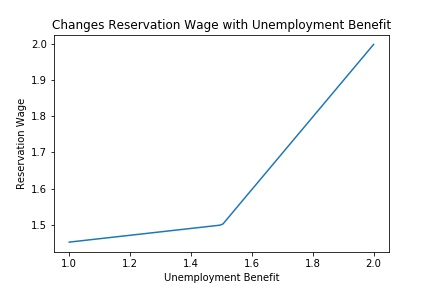
\includegraphics{rwage.jpeg}

\end{document}

